\documentclass{report}

\usepackage{fancyhdr}
\usepackage{parskip}
\usepackage{amsmath}
\usepackage[linguistics]{forest}
\usepackage[shortlabels]{enumitem}
\usepackage{float}
\usepackage{caption}
\usepackage{tikz}
\usetikzlibrary{automata, positioning, arrows}
\tikzset{
->, % makes the edges directed
>=stealth, % makes the arrow heads bold
node distance=3cm, % specifies the minimum distance between two nodes. Change if necessary.
every state/.style={thick, fill=gray!10}, % sets the properties for each ’state’ node
initial text=$ $, % sets the text that appears on the start arrow
}

\newcommand\Mydiv[2]{%
$\strut#1$\kern.25em\smash{\raise.3ex\hbox{$\big)$}}$\mkern-8mu
        \overline{\enspace\strut#2}$}

\newcommand{\doubleol}[1]{\overline{\overline{#1}}}


\pagestyle{fancy}
\fancyhf{Aaron Pierce}
\rhead{\today}
% DON'T FORGET TO CHANGE THIS vvvvvvvvvvv
\lhead{CS-3823 Homework 4}
% DON'T FORGET TO CHANGE THIS ^^^^^^^^^^^
\fancyfoot{}


\begin{document}

\section*{Problem 1(a)}
\textbf{Find the Regex for the complement language of L($\mathbf{aa^*bb^*}$)}


The essense of the regex is 1 or more $a$ followed by 1 or more $b$, so the complement is a string that has zero $a$ and/or zero $b$, or any instance of $ba$, becuase it violates the order.

So the regex is: $a^* + b^* + (a+b)^* \, ba \, (a+b)^*$

\section*{Problem 4}
\textbf{Show that if a language family is closed under union and complementation, it must also be closed under intersection.}

If $L = L_1 \cap L_2$, then $L = \doubleol{L_1 \cap L_2}$ which is $ \overline{\overline{L_1} \cup \overline{L_2}}$, by DeMorgan's law.
This is expressed using only union and complementation, which regular languages are closed over, so regular languages must also be closed under union because it can be expressed via other closed operations

\section*{Problem 10}

\textbf{Show that regular languages are closed under symmetric difference}

The symmetric difference is defined by $\left( L_1 - \left( L_1 \cap L_2 \right) \right) \cup \left( L_2 - \left( L_1 \cap L_2 \right) \right)$, creating a set of elements that are in only one of the two input sets.

Regular languages are closed under difference, as if $L = L_1 - L_2$, then $L = L_1 \cap \overline{L_2}$

We just showed that regular languages are closed under union, using the fact that they are closed under intersect and complement, so because we can represent the symmetric difference exclusively using operators unver which regular languages are closed, symmetric difference is also closed


\section*{Problem 3}

\textbf{Find an algorithm to determine whether a given regular language $\mathbf{L}$ is a palindrome language.}

The general idea is that the NFA that accepts a string in $L$ should accept its reverse, too. We know that reglangs are effectively closed under reversal, so this is possible. This is hard to show algorithmically. You can't feed every string through a machine and see if its reverse is also accepted. Instead, we'll create a machine that accepts the reverse of a language, and see if those machines define the same language. Here goes!

For an NFA $M$ that defines $L$, construct another NFA $M^R$ as follows:
\begin{enumerate}
	\item Create a copy of M and reverse all edges, call this $M^R$
	\item Add a new state $I$ and a new state $F$ to $M^R$
	\item Add epsilon transitions from $I$ to all accepting states in $M^R$
	\item Add epsilon transitions from the initial state of $M^R$ to $F$ 
	\item Designate $F$ as the only accepting state, and $I$ as the only initial state
\end{enumerate}

This generates an NFA $M^R$ which accepts $L^R$. A language is palindromic if $L(M) = L(M^R)$. This is decidable, being an instance of the equivalence problem, so you can apply the algorithm to solve the equivalence problem and decide whether or not $L$ is palindromic using this equivalence.

The equivalence problem is decidable because $L(M) = L(M^R)$ is equivalent to showing that $L(M) \subseteq L(M^R)$ and   $L(M^R) \subseteq L(M)$.
That is decidable, as we will show in problem 6.

So overall, the algorithm is to generate $M^R$ as directed above and compare it to $M$.

\section*{Problem 6}
\textbf{Show that there exists an algorithm to determine whether $\mathbf{L_1}$ is a proper subset of $\mathbf{L_2}$ for any regular languages $\mathbf{L_1}$ and $\mathbf{L_2}$.}

$L_1$ is a proper subset of $L_2$ iff $L_1 \subseteq L_2$ and $L_1 \neq L_2$. $L_1 \subseteq L_2$ is decidable, as it is equivalent to $L_1 \cap \overline{L_2} = \O$, which only uses operations that reglangs are effectively closed under. $L_1 \neq L_2$ is also decidable, as equivalence is decidable and you can take the opposite of whatever the decision is to find non-equivalence.

Equality being decidable is given by  $L(M) = L(M^R) \iff L(M) \subseteq L(M^R) \text{ and } L(M^R) \subseteq L(M)$

Thus, there exists an algorithm to determine proper subset-ness, as there exists an algorithm to determine whether $L_1$ is a subset of $L_2$ and an algorithm to determine if they are equal, both of which we have construted here.

\section*{Problem 15}
\textbf{Find an algorithm to determine whether a regular language L contains a finite number of even-length strings.}

Let $\Sigma = \left\{ \sigma_1, \sigma_2, \dots \right\}$ be the alphabet over which $L$ is constructed. 

Let $M = \left(Q, \Sigma, \delta, q_o, F \right)$  be an NFA
where $Q = \left\{ \text{init}, \text{loop}, \text{buffer} \right\}$, $q_o = \text{init}$, $F = \text{loop}$, and $\delta$ is defined as follows:

$\delta(\text{init}, \sigma) = \text{loop}$ for all $\sigma \in \Sigma$, $\delta(\text{loop}, \sigma) = \text{buffer}$ for all $\sigma \in \Sigma$,
and $\delta(\text{buffer}, \sigma) = \text{loop}$ for all $\sigma \in \Sigma$.

Why not include a diagram at this point:

\begin{figure}[H] % ’ht’ tells LaTeX to place the figure ’here’ or at the top of the page
        \centering % centers the figure
        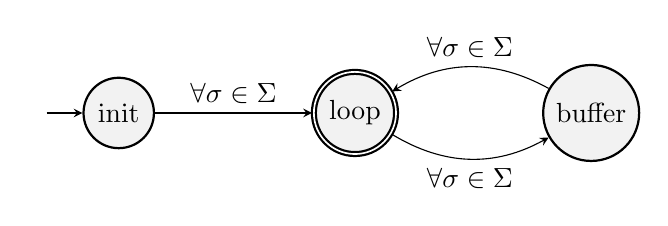
\begin{tikzpicture}

            \node[state, initial] (i) {init};
            \node[state, right of=i, accepting] (loop) {loop};
            \node[state, right of=loop] (buffer) {buffer};
            \draw   (i) edge[above] node{$\forall \sigma \in \Sigma$} (loop)
                    (loop) edge[below, bend right] node{$\forall \sigma \in \Sigma$} (buffer)
                    (buffer) edge[above, bend right] node{$\forall \sigma \in \Sigma$} (loop);
        \end{tikzpicture}
        \caption*{Call this M - it accepts any odd-length string over $\Sigma$}
        \label{fig:p3}
    \end{figure}

Let $L_\text{odd} = L(M)$, a language which consists of all odd-length strings over $\Sigma$.

A language $L$ consists of a finite number of even-length strings if $L - L_\text{odd}$ is finite, which is a decidable, accomplished via a depth-first search to identify cycles in an accepting DFA or NFA.

So because we can construct $L_\text{odd}$ which is the subset of odd-length strings from $L$, and regular languages are closed under difference, we can perform the algorithm to decide whether or not $L - L_\text{odd}$ is finite, thus deciding whether or not $L$ contains a finite number of even-length strings.

 
\section*{Problem 2}

Show that the language
\textbf{$\mathbf{L = \left\{a^n b^k c^n \, : \, n \geq 0, k \geq n\right\}}$ is not regular.}

Assume L is regular. For some value of $p$, strings of length $\geq p$ can be expressed in the form $w = xy^kz$, where $y$ is nonempty, $k \geq 0$ and $w \in L$, by the pumping lemma.


Let $w = a^n b^n c^n$. $w$ is in $L$, as $k$ can be greater than \textbf{or equal} to $n$.

You can select substrings $xyz$ in three ways:
\begin{enumerate}
\item $y$ contains only $a$'s, or $y$ contains only $c$'s
\item $y$ contains only $b$'s
\item $y$ contains both $b$'s and ($a$'s or $c$'s), or $y$ contains all three.
\end{enumerate}

In case 1, pumping $y$ more than one time will upset the balance, as there will be an unequal number of $a$'s and $c$'s

In case 3, the order will be violated. If $y$ contains two unique types of characters, then pumping $y$ multiple times will result in $a$'s coming before $b$'s, or $c$'s coming before $b$'s, which violates the structure of the language

In case 2, the exact statement of the pumping lemma becomes important. We get to pump $y$ any number of times, \textbf{including zero times}.
So if we select $y$ to contain exclusively $b$'s, then you could pump $y$ zero times, resulting in the number of $b$'s begin less than $n$.
This violates the structure.

So no matter how you choose substrings to satisfy $w = xyz$ when $w = a^n b^n c^n$, you cannot pump $y$ in a way that generates another string in $L$.

Because $w = a^n b^n c^n$ is a string in $L$, but cannot be pumped, $L$ cannot be regular.


\section*{Problem 5(c)}
\textbf{Prove the irregularity of: $\mathbf{L = \left\{a^n b^l a^k \, : \,  n = l \text{ or } l \neq k \right\}}$}


We can represent L as $L_1 \cup L_2$ where:

$L_1 = \left\{ a^n b^n a^k \right\}$ and $ L_2 = \left\{ a^n b^l a^k \, : \, n \neq k\right\}$

We know $L_1$ is not regular. $a^n b^n$ is a perfectly valid string in $L_1$, yet it cannot be pumped. Any selection of a single type of character upsets balance, choosing a substring with both $a$'s and $b$'s upsets order.

So we are unioning a potentially regular language $L_2$ with a definitely irregular language $L_1$. This will produce an irregular language.
The hypothetical NFA that could accept $L_1 \cup L_2$ will not be able to accept strings from $L_1$, but those strings are also in $L$.

Because an NFA cannot possibly accept $L_1 \cup L_2$, it must be irregular.




%%%%%
%
%     A note to the reader,
%	I spent an abhorrent amount of time on this problem. The solution was so simple and I completely
%	overlooked it trying to use the pumping lemma on it the right way.
%	I have left here all of my failed attempts at solving this problem, maintaining exactly the character I left off from,
%	so that you may experience each individual train of thought derailing as I endured for hours.
% 	It's really not that much, but let me tell you: it felt like much.
%
%%%%%
%%%	
%%%	\noindent\makebox[\linewidth]{\rule{\paperwidth}{0.4pt}}
%%%	
%%%	
%%%	I'll spare you the repetition of the pumping lemma which I just spit out last problem.
%%%	The key is that given \textbf{any} string in $L$, we can pump it \textbf{zero or more} times to make another string in $L$.
%%%	
%%%	So if you hand me $a^{n}$, for some sufficiently large $n$, the string is in $L$ but I cannot pump any of its substrings.
%%%	
%%%	The string is in $L$ by setting $n=n$, $l=0$ and $k = 0$, but when I want to pump the only thing I can select is some number of $a$'s.
%%%	
%%%	No matter how many times I repeat $a$, it will always be true that $l = k$, because they are both 0.
%%%	
%%%	Sure, you could pump the entirety of $a^n$ 0 times, so the string is empty, which is a string in $L$, but you need to be able to pump it any amount of times you want, so any value other than $0$ generates a string that is not in $L$.
%%%	
%%%	Becuase there is no substring of $a^n$ any number of times that can be pumped 
%%%	
%%%	\noindent\makebox[\linewidth]{\rule{\paperwidth}{0.4pt}}
%%%	
%%%	
%%%	I'll spare you the repetition of the pumping lemma which I just spit out last problem.
%%%	The key is that given \textbf{any} string in $L$, we can pump it \textbf{zero or more} times to make another string in $L$.
%%%	
%%%	So if you hand me $a^{v+1} b^v a^{v+1}$, for some sufficiently large $v$, the string is in $L$ but I cannot pump any of its substrings.
%%%	
%%%	If my pumping substring contains both $a$'s and $b$'s, pumping it multiple times violates the order of the string, so my pumping string must exclusively consist of $a$'s or $b$'s.
%%%	
%%%	If my substring comes exclusively from the first term, $a^n$, then pumping it more than zero times will result in $n > l$, which violates $n = l$.
%%%	
%%%	If my substring comes exclusively from the middle term, $b^l$, then I could pump a single character for it to generate a string in $L$, but I need to be able to pump it an arbitrary amount of times. Pumping it any number of times more than $1$ results in 
%%%	
%%%	
%%%	\noindent\makebox[\linewidth]{\rule{\paperwidth}{0.4pt}}
%%%	
%%%	I'll spare you the repetition of the pumping lemma which I just spit out last problem.
%%%	The key is that given \textbf{any} string in $L$, we can pump it \textbf{zero or more} times to make another string in $L$.
%%%	
%%%	So if you hand me $a^n b^l$, you have handed me a string in $L$ where $k = 0$.
%%%	
%%%	I cannot pump this string. I either need to achieve $n = l$ or $l \neq k$
%%%	
%%%	If my goal is to pump $n$ to equal $l$ I can't do it. If my pumping string has both symbols in it the order will be violated, and if it doesn't I can pump one string
%%%	$l + 1$ times and it's over. They can't possibly be equal.
%%%	
%%%	If my goal is to pump so that $l \neq k$, that's a little easier. I just pump the $a^n$ part freely, right?
%%%	
%%%	Wrong. Take a look at the string $a^n b^l a^l$.
%%%	
%%%	If my substring contains only symbols beloi
%%%	
%%%	
%%%	\subsection*{Big case 1: $\mathbf{n = l}$}
%%%	When $n = l$ you can just select any section of $a^k$ to be your pumping string, which will generate more strings in $L$, which makes this language smell a little regular. 
%%%	However, $k$ can be 0, and you can't pump a zero-length string.
%%%	
%%%	But it gets deeper, if $k = 0$ and $n = l$ then $l$ must be greater than 0 in order for the total string length to be greater than our pumping constant, so it must be the case that $l \neq k$, which forms...
%%%	
%%%	\subsection*{Big case 2: $\mathbf{l \neq k}$} 
%%%	
%%%	When $l \neq k$, we must show that any substring can be pumped to force $l$ to equal $k$.
%%%	
%%%	There are two subcases to consider. First, you don't want to include any part of $a^k$ in your pumping substring because that will obviously ruin your chances of making $l = k$, which is our strategy in this contradiction, so we can safely ignore that case.
%%%	
%%%	So we arrive at.
%%%	
%%%	\subsubsection*{Big case 2 subcase 1: your pumping string contains only symbols from $\mathbf{a^n}$}




\end{document}